\section{Architecture}
The following section discusses the architecture of the deep neural network generated by ZyNet, its parameters and application interface.
\subsection{Neuron}
\begin{figure}[!t]
\centering
   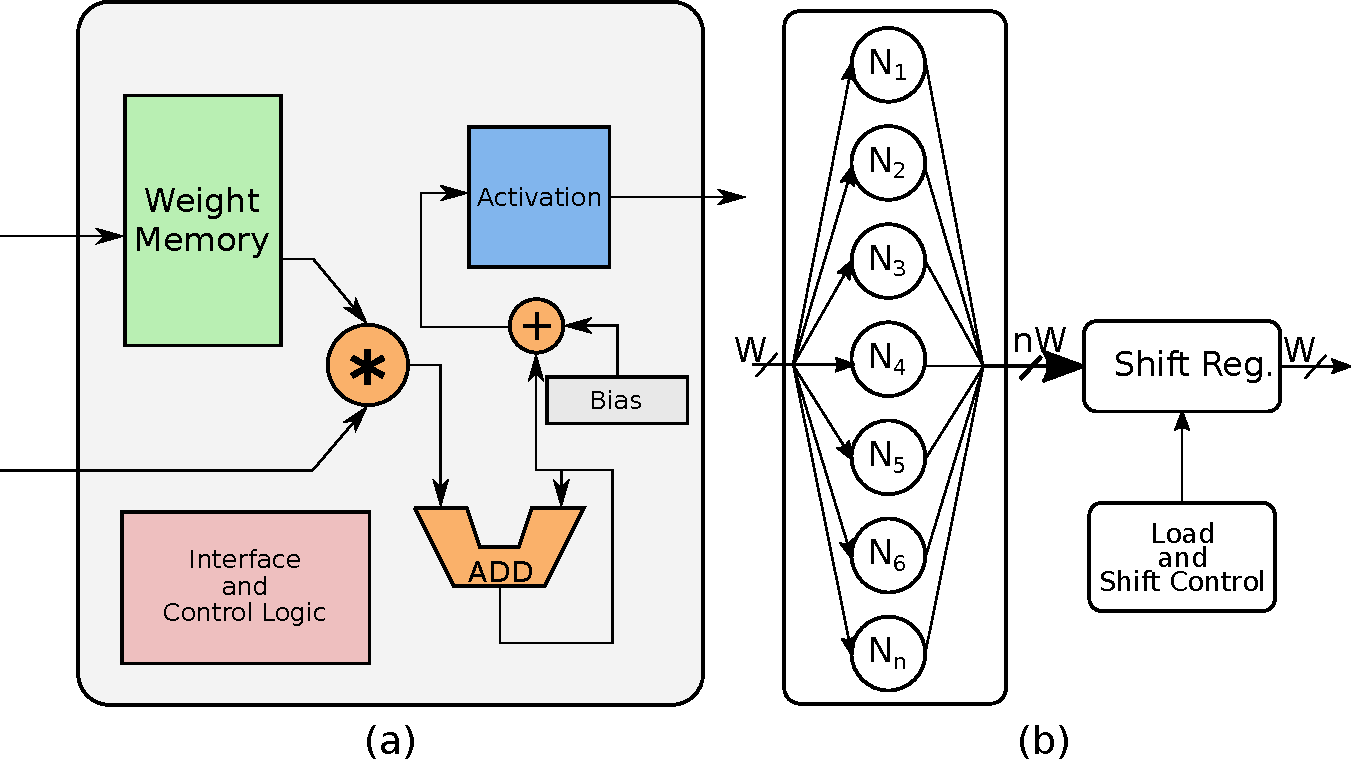
\includegraphics[width=\columnwidth]{Figures/neuron.pdf}
   \caption{Neuron Architecture}
   \label{fig:neuron}
   \vspace{-3mm}
\end{figure}
The architecture of a single artificial neuron is as shown in Fig.~\ref{fig:neuron}.
Each neuron has independent interfaces for configuration (weight, bias etc.) and for streaming data in and out.
Irrespective of number of neighbors, each neuron has a single interface for accepting data.
This enables scalability of the network and improves clock performance by compromising on latency. 

An internal memory, whose size is decided by the number of inputs to the neuron, is used to store the weight values corresponding to each input.
Depending on whether the network is configured as \emph{pre-trained} or not, either a RAM with read and write interface or a ROM initialized with weight values are instantiated.
As inputs are streamed into the neuron, a control logic reads the corresponding weight value from the memory.
Inputs and corresponding weight values are multiplied and accumulated (MAC) and finally added with the \emph{bias} value.
Like the weights, the bias value is stored in a register at implementation time if the network is \emph{pre-trained} or configured at run-time with software.
The output from the MAC unit is finally applied to the activation unit.
Based on the type of activation function configured (Sigmoid, ReLU, hardMax etc.), either a look-up-table based (for Sigmoid) or a circuit-based function is implemented by the tool.
The type of function chosen has a direct impact on the accuracy of the network and the total resource utilization and clock performance. 

\subsection{Layer}
Each layer instantiates user specified number of neurons and manages data movement between the layers.
Since each neuron has a single data interface and a fully connected layer requires connection to every neuron in the previous layer, data from each layer is initially stored in a shift register.
It is then shifted to the next layer one per clock cycle.

\subsection{System Architecture}
Fig.~\ref{fig:sysarch} depicts the complete system architecture generated by ZyNet when targeting the Zynq platform.
It packages ZyNet as an IP core and automatically integrates with other peripherals.
The AXI4-Lite interface of ZyNet is connected to the GP0~(General Purpose) interface of Zynq PS~(processing system).
This interface is used for configuration in case of untrained networks and for reading out the final network output in case of both pre-trained and untrained network.

The streaming interface from ZyNet is connected to a DMA controller, which in turn is connected to the external memory through the Zynq HP0 (high performance) interface.
This enables training and test data to be directly streamed from external memory to ZyNet.
The DMA controller is also interfaced with the Zynq GP port for configuration.
Interrupt signals from both ZyNet and DMA controller are connected to the PS interrupt interface.
 
\begin{figure}[!t]
\centering
   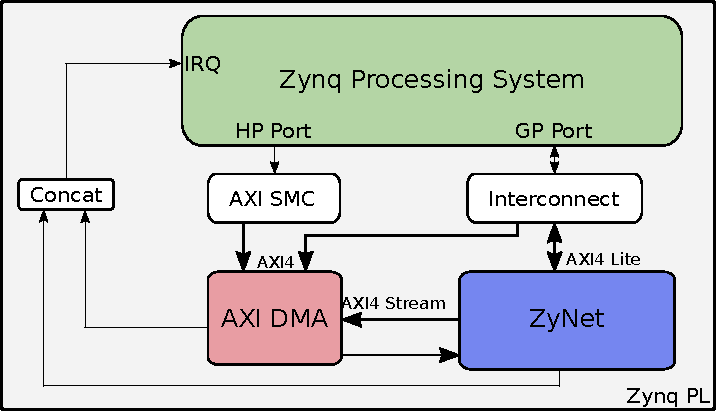
\includegraphics[width=0.8\columnwidth]{Figures/arch.pdf}
   \caption{System Architecture}
   \label{fig:sysarch}
\end{figure}


\subsection{APIs}

\begin{table}[!h]
  \centering
  \caption{Important methods available in the ZyNet package} 
  \begin{tabular}{l|l}
      \toprule
      \bf{Methods} & \bf{Action} \\
      \midrule
	zynet.model() & Creates a zynet DNN object \\
	model.add() & Adds a new layer to the DNN \\
	model.compile() & Generates the DNN RTL code\\
	zynet.makeXilinxProject() & Generates a Xilinx project\\ 
				  & with DNN as the top module\\
	zynet.makeIP() & Packeges the DNN into IP-XACT format\\
	zynet.makeSystem & Creates a block design with the generated \\
			 & IP block, Zynq processor system,\\ 
			 & DMA controller and other peripherals\\
      \bottomrule
    \end{tabular}
    \label{table:apis}
\end{table}
